\section{Experimental Results}
\label{sec:experimentalResults}

\subsection{3D Laser Scanning}
\label{sec:experimentalResults:3DLaserScanning}

The test of the 3D laser scanning consists of 3 phases.
First a semi stationary scan is performed by moving the robot manually in a limited manner (tilting it by approximately $\SI{45}{\degree}$) without its exterior shell.
This results in the 3D point cloud in figure \ref{sec:experimentalResults:3DLaserScanning:fig:firstpointcloud}.
For the second test the same movement is used.
However, this time the outside shell of the robot is present.
This results in figure \ref{sec:experimentalResults:3DLaserScanning:fig:secondpointcloud}.
Finally, the COAM-drive enabled test of the overall system leads to a 3D point cloud consisting of multiple revolutions.
Figure \ref{sec:experimentalResults:3DLaserScanning:fig:thirdpointcloud} shows results.

\todo{Point size increase, maybe black on white? }
\begin{figure}
\centering
\begin{subfigure}[b]{0.49\textwidth}
	\centering
	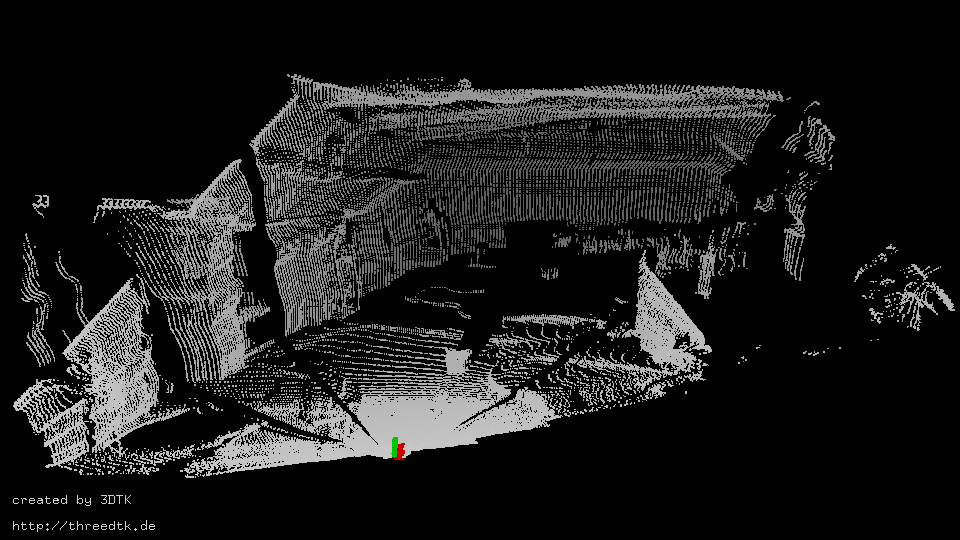
\includegraphics[width=\textwidth,trim={0 1cm 0 1cm},clip]{../Media/FirstDecentMap}
	\caption{Test with limited movement and no exterior shell.}
	\label{sec:experimentalResults:3DLaserScanning:fig:firstpointcloud}
\end{subfigure}
\hfill
\begin{subfigure}[b]{0.49\textwidth}
	\centering
	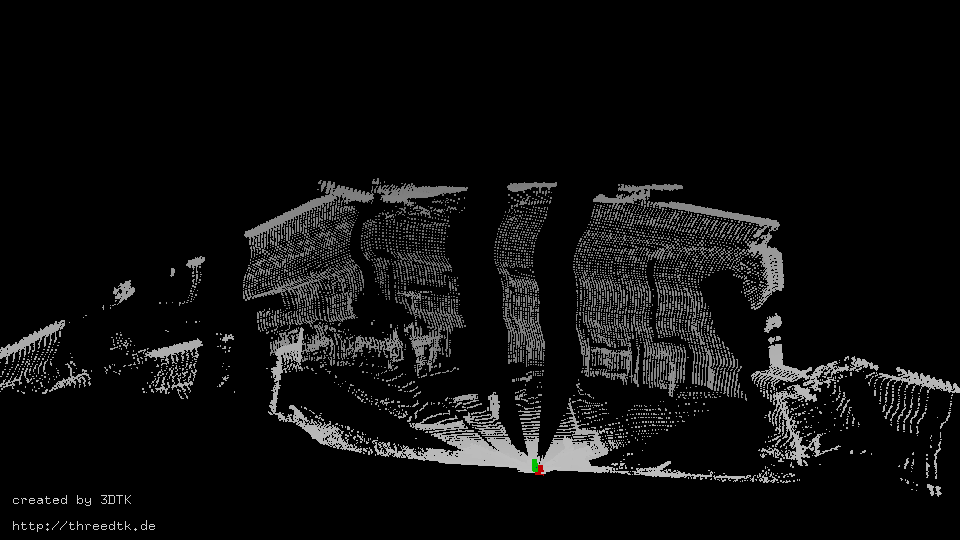
\includegraphics[width=\textwidth,trim={0 1cm 0 1cm},clip]{../Media/testScanWithTop}
	\caption{Test with limited movement but present exterior shell.}
	\label{sec:experimentalResults:3DLaserScanning:fig:secondpointcloud}
\end{subfigure}
\\
\begin{subfigure}[b]{\textwidth}
	\centering
	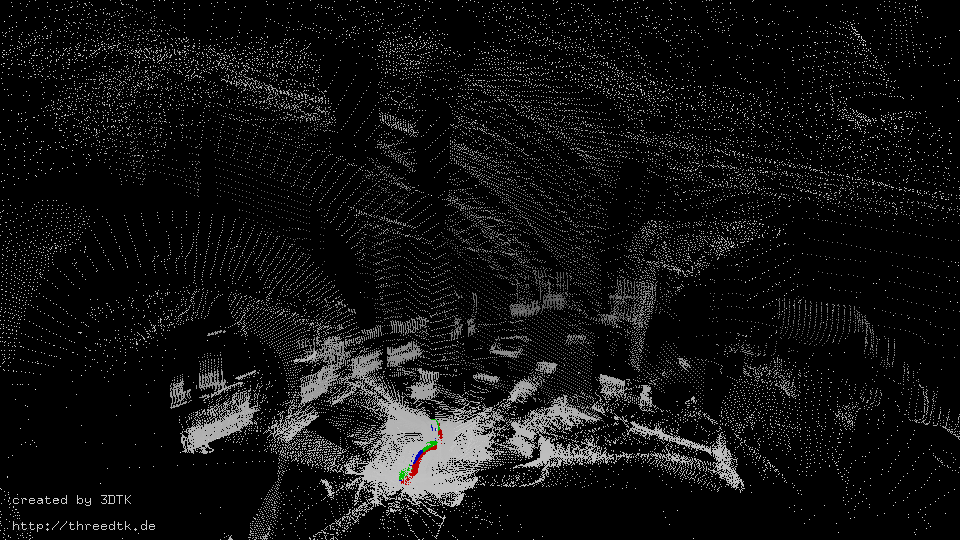
\includegraphics[width=\textwidth,trim={0 1cm 0 1cm},clip]{../Media/RollingTestMap}
	\caption{Test with exterior shell and full movement (i.e. multiple revolutions).}
	\label{sec:experimentalResults:3DLaserScanning:fig:thirdpointcloud}
\end{subfigure}
\caption{3D Point cloud results of different test scenarios of the system.}
\end{figure}

The first test yields the clearest 3D point cloud (figure \ref{sec:experimentalResults:3DLaserScanning:fig:firstpointcloud}).
This is contributed to the fact, that in this test the exterior shell is absent.
Since the shell partially reflects the beams of the laser scanner, the noise level increases.
In this case the laser scanner measures the shell instead of the environment around it.
In figure \ref{sec:experimentalResults:3DLaserScanning:fig:secondpointcloud} lines are blocked that are measured in the previous test further showing the reflection of the laser beams by the shell.
The rolling motion of the robot increases this effect.
Specifically, a large number of measurement points along the path of the robot manifests this (figure \ref{sec:experimentalResults:3DLaserScanning:fig:thirdpointcloud}).
We assume that the more powerfull laser scanner LMS141 reduces this effect. 

Furthermore, the time asynchrony of the pose determination sub-system and the laser scanner introduces further systematic errors to the 3D point cloud.
Specifically, figure \ref{sec:experimentalResults:3DLaserScanning:fig:thirdpointcloud} shows that the laser scanner detects points underneath the surface the robot was rolling on. 

\subsection{COAM Drive}
\label{sec:experimentalResults:COAMDrive}

The conversation of angular momentum drive accelerates the L.U.N.A. sphere reliably.
Figure \ref{sec:experimentalResults:COAMDrive:fig:angvel} shows the angular acceleration of the whole sphere measured by the IMU system in one test run. Furthermore, it shows that the acceleration along the rotational axis of the flywheels rises while the accelerations along the other axes remain lower, albeit are noisy.
The vibrations and tilt of the robot contribute to the velocities along the other axes.
The vibrations are results of inexact drilling of the flywheels such that there is an unbalance.
At the main test site the ground is a hard, clean and low friction concrete floor.
In such a scenario the vibrations add up and lead to slippage.
However, a rubber surface (a running track) absorb the vibrations, such that the acceleration process happens reliably.

\todo{Vergleich mit 1 IMU machen, evtl rauschen zeigen}

\begin{figure}
\centering
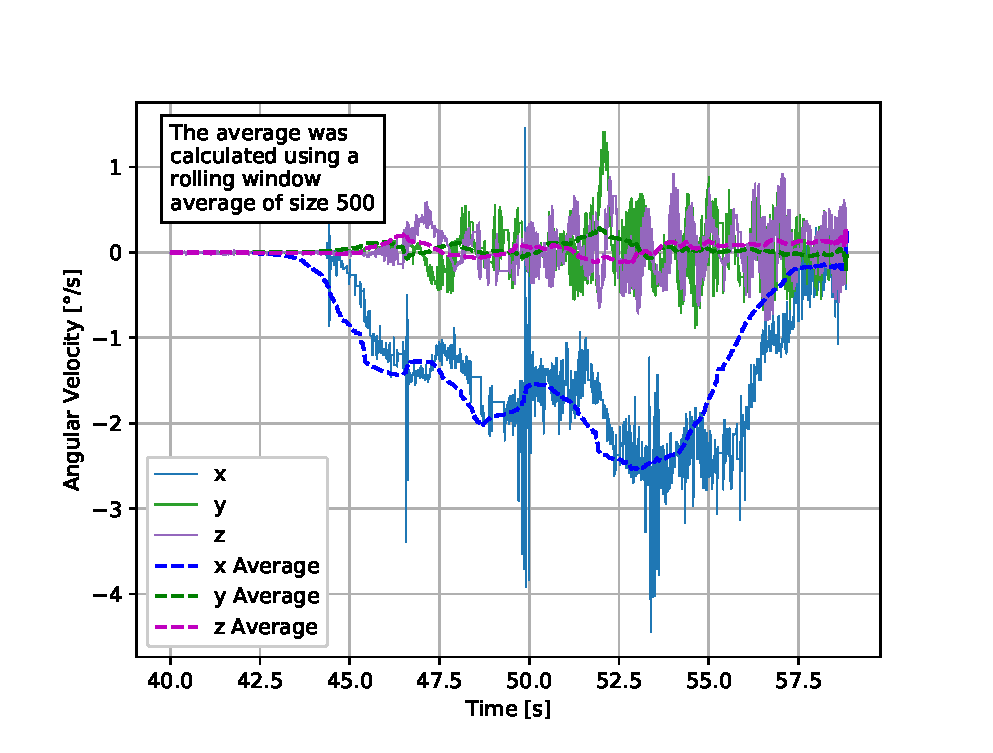
\includegraphics[width=\textwidth]{./plotsAndScripts/angVel-2020-01-29-16-14-54/ang-vel}
\caption{Angular velocities of the L.U.N.A. - sphere during a test run. The flywheels rotate around the x-axis in positive direction. Velocities in the other direction can mostly be contributed to vibrations and tilt of the robot.}
\label{sec:experimentalResults:COAMDrive:fig:angvel}
\end{figure}